\documentclass[a4paper]{article}
\usepackage[14pt]{extsizes}
\usepackage[utf8]{inputenc}
\usepackage[T2A]{fontenc}
\usepackage[russian]{babel}
\usepackage{setspace,amsmath}
\usepackage{amssymb, amsthm}
\usepackage{graphicx}
\usepackage{mathtext}
\usepackage{mathenv}
\usepackage{tocloft}
\usepackage{enumitem}
\usepackage{array}
\usepackage{lipsum}
\usepackage[indentfirst]{titlesec}
\usepackage[left=30mm, top=20mm, right=20mm, bottom=20mm, nohead, footskip=10mm]{geometry}


\onehalfspacing

\makeatletter
\renewcommand{\cftsecleader}{\cftdotfill{\cftdotsep}}

\newtheorem*{mproblem}{Условие}
\newtheorem*{mclaim}{Утверждение}
\newtheorem*{mremark}{Замечание}
\newtheorem*{mdefinition}{Определение}
\newtheorem*{mlemma}{Лемма}
\newtheorem*{mtheorem}{Теорема}
\newtheorem*{msolution}{Доказательство}
\newtheorem*{mexample}{Пример}

\begin{document}
\begin{titlepage}
	\begin{center}
		\hfill \break
		\large{Министерство образования и науки Российской Федерации}\\
		\hfill \break
		\normalsize{Государственное образовательное учреждение}\\ 
		\normalsize{высшего профессионального образования}\\
		\normalsize{«Московский физико-технический институт (государственный университет)»}\\
		\normalsize{Факультет инноваций и высоких технологий}\\
		\normalsize{Кафедра анализа данных}\\
		\hfill \break
		\hfill \break
		\hfill \break
		\Large{\textbf{Магистерская диссертация}}\\
		\hfill \break
		\large{Тема: \textbf{Название моей работы (TODO)}}\\
	\end{center}

	\begin{flushright}
		\hfill \break
		Направление:  010400\\
		Прикладные математика и информатика\\
		\hfill \break
		\hfill \break
		\hfill \break
	\end{flushright}
	
	\begin{flushright}
		\normalsize{
			\begin{tabular}{rcr}
				Выполнил:\ \\ студент 093 группы & \underline{\hspace{3cm}} & Попов М.В. \\\\
				Научный руководитель:\ \\ д.физ.-мат.н., проф.(todo) & \underline{\hspace{3cm}}& Ромащенко А.Е. \\\\
			\end{tabular}
		}
	\end{flushright}

	\begin{center}
		\hfill \break
	\end{center}

	\begin{center} г. Москва 2016 \end{center}
	\thispagestyle{empty}
\end{titlepage}
 
\newpage

\tableofcontents

\newpage
 
\newpage


\setcounter{section}{0}
\section*{Введение}
\addcontentsline{toc}{section}{Введение}
(ToDo) Актуальность, новизна, краткая выжимка.

\addtocounter{section}{1}
\section*{Коммуникационная сложность}
\addcontentsline{toc}{section}{Коммуникационная сложность}
\setcounter{subsection}{0}

\subsection{Постановка задачи}
Мы будем рассматривать задачи следующего вида: пусть имеются два человека, которые хотят совместно
вычислить значение некоторой функции от двух переменных $f(x, y)$. По традиции мы будем называть
первого участника игры Алисой, а второго -- Бобом. Сложность у этой задачи в том, что Алиса знает только
значение аргумента $x$, а Боб значение аргумента $y$. Алиса и Боб могут обмениваться сообщениями 
по каналу связи. Требуется вычислить значение $f(x, y)$, переслав по каналу связи минимальное
количество информации.

Мы предполагаем, что Алиса и Боб заранее (до того, как им станут известны значения $x$ и $y$)
договариваются о коммуникационном протоколе --- о наборе соглашений, какие именно данные и
в каком порядке они будут пересылать друг другу при тех или иных значениях $x$ и $y$.

Опишем теперь всю задачу более формально. Пусть имеются конечные множества $X, Y, Z$ и задана
некоторая функция $f:X\times Y\rightarrow Z$.

\begin{mdefinition}
    Коммуникационным протоколом для вычисления некоторой функции $f:X\times Y\rightarrow Z$ называется
    ориентированное двоичное дерево со следующей разметкой на вершинах и ребрах:
    \begin{itemize}[noitemsep]
        \item каждая нелистовая вершина помечена буквой $A$ или $B$;
        \begin{itemize}[noitemsep]
			\item у вершин с пометкой $A$ определена функция $g_i:X\rightarrow \{0,1\}$;
			\item у вершин с пометкой $B$ определена функция $f_j:Y\rightarrow \{0,1\}$;
        \end{itemize}
        \item каждой листовой вершине сопоставлен элемент множеста $Z$;
        \item каждое ребро помечено $0$ или $1$.

    \end{itemize}
\end{mdefinition}

Пусть Алиса и Боб договорились, что будут действовать по некоторому протоколу $\mathcal{P}$. Затем
Алиса получила $x\in X$, а Боб получил $y\in Y$. Поместим фишку в корневую вершину нашего протокола
$\mathcal{P}$ и будем перемещать ее вниз по дереву, последовательно удаляясь от корня,
пока она не попадет в один из листьев. Перемещение фишки выполняется следующим образом. Если текущая 
вершина помечена буквой $A$, то это означает, что сейчас очередь Алисы. Она применяет функцию $g_i$ текущей 
вершины к своему значению $x$. Алиса отправляет по каналу связи бит равный $g_i(x)$ и перемещает
фишку по ребру, помеченному как $g_i(x)$. Боб получает отправленный бит и понимает куда была сдвинута фишка.
Для вершин помеченных буквой $B$ эту же процедуру выполняет Боб. Когда фишка попадает в лист дерева,
записанное там значение $z\in Z$, объявляется результатом выполнения протокола.

Мы говорим, что протокол $\mathcal{P}$ вычисляет функцию $f:X\times Y \rightarrow Z$, если для любого
$x\in X$ и любого $y\in Y$ при движении из корня по пути, соответствующему заданным $x$ и $y$,
мы попадаем в лист, помеченный $z=f(x,y)$.

\begin{mdefinition}
	Сложностью коммуникационного протокола называется его глубина. Коммуникационной сложностью функции 
	$f$ называется минимальная сложность протокола, вычисляющего $f$. Мы будем обозначать её $CC(f)$.
\end{mdefinition}


\subsection{Одноцветные комбинаторные прямоугольники}
\begin{mdefinition}
	Множество $S \subseteq X\times Y$ называется комбинаторным прямоугольником (или просто прямоугольным
	множеством), если существуют такие $A \subseteq X$ и $B \subseteq Y$, что $S = A\times B$.
\end{mdefinition}

Пусть $\mathcal{P}$ -- некоторый коммуникационный протокол для вычисления функции $f:X\times Y \rightarrow Z$ 
и $l$ -- один из листьев протокола. Определим $S_l$ как множество пар $(x, y) \in X\times Y$ таких, что 
на входе $(x,y)$ Алиса и Боб, следуя протоколу $\mathcal{P}$, приходят в лист $l$.

\begin{mclaim}
    Для всякого коммуникационного протокола $\mathcal{P}$ и для всякого листа $l$ множество $S_l$
    является комбинаторным прямоугольником. 
\end{mclaim}

Доказательство этого утверждения можно прочитать, например, в \cite{KushilevitzNisan}. В итоге мы получаем,
что коммуникационный протокол для вычисления функции $f$ задаёт разбиение $X\times Y$ - 
таблицы значений $f$ на прямоугольные множества, соответствующие листьям. Поскольку каждому
листу протокола приписано одно значение функции $f$, эти прямоугольные множества являются одноцветными,
то есть во всех точках такого прямоугольного множества функция $f$ принимает одно и то же значение.
Например, для $X = Y = \{1, 2, 3, 4\}$, $Z = \{0, 1\}$ и протокола $\mathcal{P}$ (рис. 1) получаем 
разбиение на $5$ одноцветных прямоугольных множеств. 

\begin{figure}
	\centering
	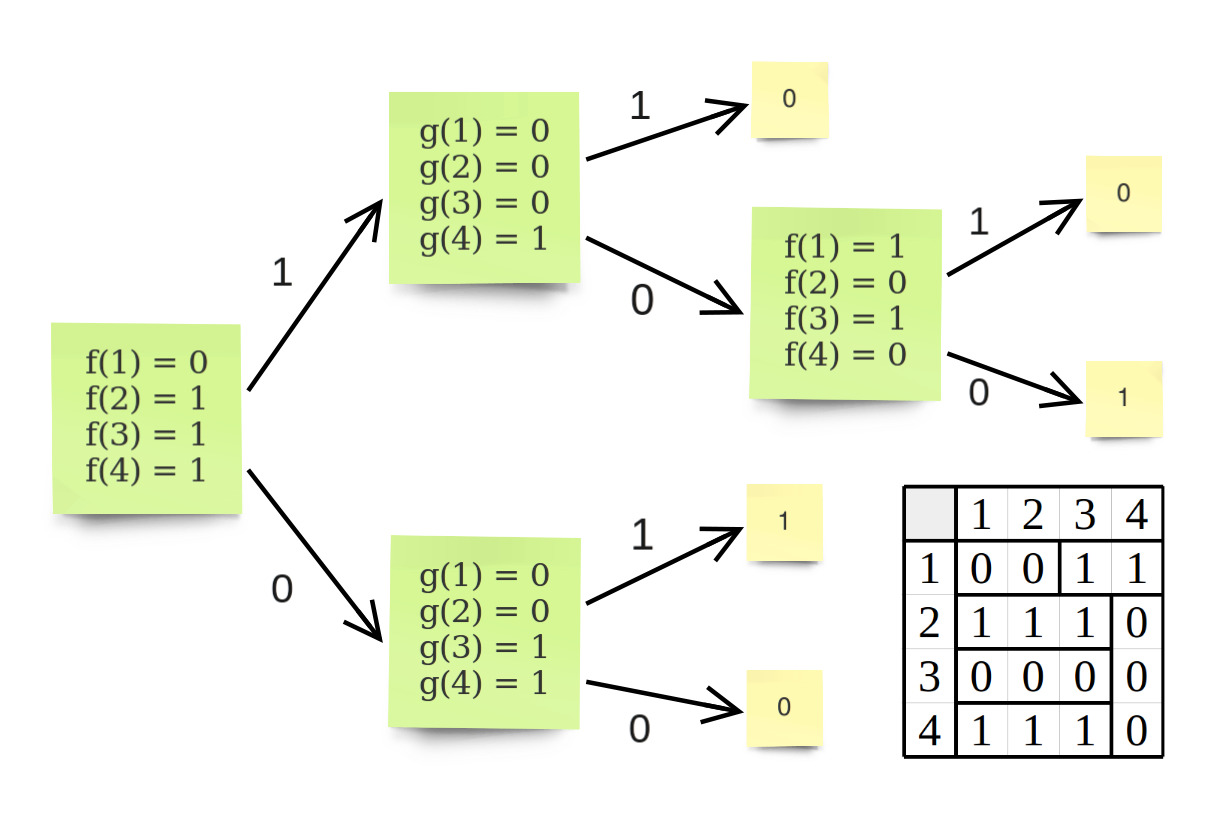
\includegraphics[width=0.8\textwidth]{images/protocol.png}
	\caption{Пример протокола и разбиения таблицы значений.}
\end{figure}

Подведем промежуточные итоги: всякий протокол с $l$ листьями (вычисляющий функцию $f$) задаёт разбиение
таблицы значений $f$ на $l$ одноцветных прямоугольных множеств. Значит, чтобы доказать, что коммуникационная 
сложность $CC(f)$ не меньше $n$, достаточно показать, что таблицу значений невозможно разбить на менее,
чем $2^n$ одноцветных прямоугольных множеств.

\subsection{Графовая интерпретация}

Давайте теперь посмотрим на другое представление множества значений функции $f$. Рассмотрим полный 
двудольный граф $G = (X, Y, E)$, ребра которого раскрашены в $|Z|$ цветов. Вершины левой доли 
соответствуют элементам множества $X$, вершины правой доли - элементам множества $Y$. Ребро 
$(x, y) \in X\times Y$ имеет цвет $z \in Z$, если $f(x, y) = z$.

Из определения комбинаторного прямоугольника видно, что в графовой интерпертации он является ничем
иным, как полным двудольным подграфом. А разбиение таблицы значений $f$ на одноцветные прямоугольные
множества -- это разбиение нашего  полного двудольного графа $G$ на одноцветные непересекающиеся биклики 
(полные двудольные подграфы). Для нашего примера графовую интерпретацию можно посмотреть на рис. 2.

\begin{figure}
	\centering
	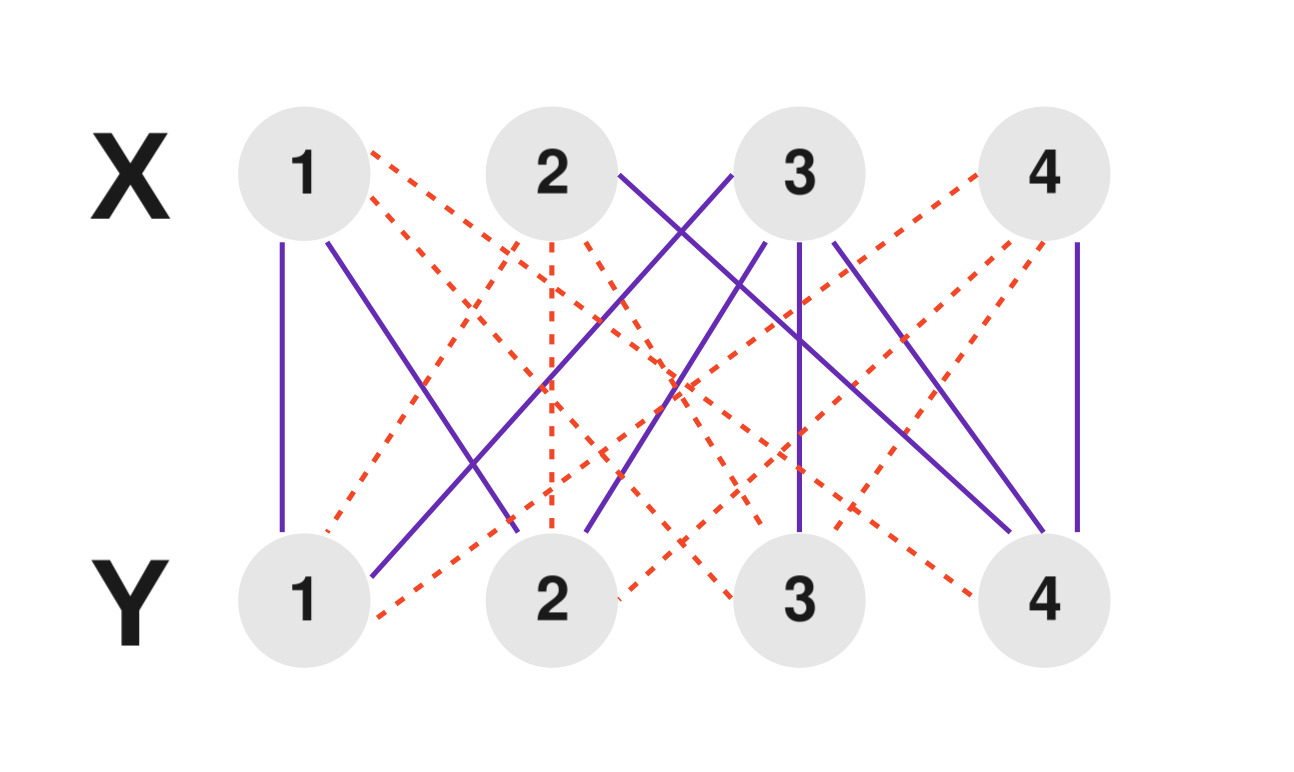
\includegraphics[width=0.6\textwidth]{images/biclique.png}
	\caption{Графовая интерпретация: синие -- 0, красные -- 1.}
\end{figure}

\begin{mdefinition}
	Бикликовым разбиением $bcp(G)$ двудольного графа $G$ будем называть наименьшее число непересекающихся
	биклик, которыми можно покрыть все ребра графа $G$.
\end{mdefinition}


\begin{mdefinition}
	Бикликовым покрытием $bcc(G)$ двудольного графа $G$ будем называть наименьшее число, возможно, 
	пересекающихся биклик, которыми можно покрыть все ребра графа $G$.
\end{mdefinition}

\begin{mclaim}
    Для произвольного двудольного графа $G$ верно $$bcp(G) \geq bcc(G)$$
\end{mclaim}

Для каждого $z \in Z$ определим двудольный граф $G_z = (X, Y, E_z)$, как граф, получающийся из $G$ 
выкидыванием всех ребер цвета, отличного от $z$. Иначе говоря $E_z = \{(x,y)\in X\times Y\ |\ f(x, y) = z \}$.

Величины $bcp(G_z)$ и $bcc(G_z)$ дают некоторую нижнюю оценку на коммуникационную сложность функции $f$, 
с которой намного удобнее работать: $$2^{CC(f)}\geq \sum\limits_{z\in Z}bcp(G_z)\geq \sum\limits_{z\in Z}bcc(G_z)$$

\begin{mremark}
    На самом деле величины $bcc(G_z)$ тесно связаны с недетерминированной коммуникационной сложностью 
    $NCC(f)$. Для произвольного множества $Z$ верно:
    \begin{itemize}[noitemsep]
        \item $2^{NCC(f)}\geq \sum\limits_{z\in Z}bcc(G_z)$,
        \item $NCC(f) \leq \lceil \log_2(\sum\limits_{z\in Z}bcc(G_z))\rceil + 1$
    \end{itemize}
    Иначе говоря, величины $bcc(G_z)$ и $NCC(f)$ по существу задают одну и ту же меру "сложности"\ функции $f$. 
    Подробнее про это можно прочитать, например, в \cite{Razborov}.
\end{mremark}

В итоге мы получили мощный иструмент для доказательства нижних оценок коммуникационной сложности. 
К сожалению, задача нахождения величины $bcc(G)$ является PSPACE-полной \cite{HermannMarkus}, а точное 
значение известно только для очень скудного класса графов (например, для "crown graphs"\ \cite{CrownGraph}), поэтому 
напрямую мы не можем использовать эту оценку. В следующей главе я рассмотрю несколько методов, 
позволяющих для произвольного двудольного графа оценивать снизу величину $bcc(G)$.


\addtocounter{section}{1}
\section*{Оценивание $bcc(G)$}
\addcontentsline{toc}{section}{Оценивание $bcc(G)$}

В этой главе я опишу три различных метода оценивания бикликового покрытия:
\begin{itemize}[noitemsep]
	\item метод трудного множества ("fooling set");
	\item метод Куликова-Юкны;
	\item метод энтропийных неравенств.
\end{itemize}

Первые два метода работают для произвольных графов (необязательно двудольных), а третий применим к 
большому классу двудольных графов.

\setcounter{subsection}{0}

\subsection{Метод трудного множества}

Данный метод тесно связан с одноцветными прямоугольными множествами. Классическое определение 
трудного множества выглядит следующим образом:

\begin{mdefinition}
	Для функции $f: X\times Y \rightarrow Z$ и элемента $z\in Z$ будем называть множество 
	$S_z\subset X\times Y$ трудным (в англоязычной литературе fooling set), если верно:
	\begin{itemize}[noitemsep]
		\item для всякой пары $(x, y)\in S_z$ имеем $f(x, y) = z$;
		\item для любых двух несовпадающих пар $(x, y)\in S_z$ и $(x', y')\in S_z$ имеем 
		$f(x, y') \neq z$ или $f(x', y) \neq z$.
	\end{itemize}
\end{mdefinition}

Нас будет интересовать немного более общее определение трудного множества (графовая интерпретация):
\begin{mdefinition}
	Пусть $G = (V, E)$ произвольный неориентированный граф. Будем называть подмножество ребер 
	$S \subseteq E$ трудным, если для любых двух различных ребер $(x, y)\in S$ и $(x', y')\in S$ 
	имеем $(x, y') \notin E$ или $(x', y) \notin E$. Обозначение $fool(G)$ - размер максимального по 
	мощности трудного множества.
\end{mdefinition}

\begin{mremark}
	Классическое определение получается из графового, применением к двудольному графу $G_z = (X, Y, E_z)$, 
	который строится по функции $f: X\times Y \rightarrow Z$.
\end{mremark}

	
\begin{mtheorem}
    Для произвольного неориентированного графа $G = (V, E)$, если подмножество ребер $S \subseteq E$ 
    является трудным, то $bcc(G) \geq |S|$.
\end{mtheorem}

\begin{msolution}
    Достаточно доказать, что два ребра, лежащие одновременно в одном трудном множестве, не могут 
    попасть в одну биклику. Пусть не так, значит существуют два ребра $(x, y)\in B\cap S$ и 
    $(x', y')\in B\cap S$, где $B$ - биклика, а $S$ - трудное подмножество ребер. Но тогда ребра 
    $(x, y')$ и $(x', y)$ также принадлежат биклике $B$, а значит лежат и в нашем множестве ребер 
    $E$. Противоречие. $\blacksquare$
\end{msolution}

\subsection{Метод Куликова-Юкны}
Следующий метод был впервые описан в статье \cite{KulikovJukna}, и работает он для произвольного 
неориентированного графа.

\begin{mtheorem}
    Для произвольного неориентированного графа $G = (V, E)$ верно: $$bcc(G)\geq \left\lceil\frac{v(G)^2}{|E|}\right\rceil$$ 
    где $v(G)$ -- размер максимального паросочетания графа $G$.
\end{mtheorem}

\begin{msolution}
	Пусть $M\subseteq E$ - это максимальное паросочетание, тогда рассмотрим бикликовое покрытие, 
	на котором достигается минимум $E = B_1\cup B_2\cup \ldots \cup B_{bcc(G)}$. Определим 
	отображение $g:M\rightarrow \{1,\ \ldots,\ bcc(G)\}$, как $g(e) = min\{i\ |\ e\in B_i\}$ и пусть 
	$M_i = \{e\in M\ |\ g(e) = i\}$. Иначе говоря $M_i$ содержит только те ребра максимального 
	паросочетания $M$, которые покрываются бикликой $B_i$ впервый раз.
	
	Пусть $F_i \subseteq B_i$ биклика, индуцированная вершинами ребер из $M_i$. Пусть 
	$F = F_1\sqcup F_2\sqcup \ldots \sqcup F_{bcc(G)}$ (биклики $F_i$ не пересекаются по построению).
	
	Очевидно, что $F_i$ - биклика размера $r_i\times r_i$, где $r_i = |M_i|$. Получаем следующие 
	соотношения: $$r_1 + r_2 + \ldots + r_{bcc(G)} = |M| = v(G)$$ и 
	$$r_1^2 + r_2^2 + \ldots + r_{bcc(G)}^2 = |F|$$ Из неравенства Коши-Буняковского получаем 
	$$v(G)^2 = (r_1 + r_2 + \ldots + r_{bcc(G)})^2 \leq bcc(G)\cdot (r_1^2 + r_2^2 + \ldots + r_{bcc(G)}^2) = bcc(G)\cdot |F|$$
	А так как $F \subseteq E$, то $$v(G)^2\leq bcc(G)\cdot |F| \leq bcc(G)\cdot |E|\ \blacksquare$$

\end{msolution}

В этой же статье \cite{KulikovJukna} этот метод сравнивался с другой оценкой: пусть $bcl(G) = \max\limits_{K_{r,r}\subseteq G}\{r\}$, 
тогда
\[bcc(G) \geq \left\lceil\frac{v(G)}{bcl(G)}\right\rceil \tag{*}\]
Данная оценка очевидным образом следует из того, что любая биклика $K_{r, s}$ содержит как максимум 
$min\{r, s\}$ ребер максимального паросочетания.

Приведем примеры графов, на которых метод Куликова-Юкны работает намного лучше, чем оценка (*), и наоборот:

\begin{itemize}
    \item пусть двудольный граф $G = (L, R, E)$ состоит из совершенного паросочетания размера 
    $n = |L| = |R|$ и еще некоторого константного числа непересекающихся биклик $K_{r,r}$. 
    К тому же, пусть $r = \Theta(\sqrt{n})$, тогда $$\left\lceil\frac{v(G)^2}{|E|}\right\rceil = 
    \left\lceil\frac{n^2}{cr^2 + n}\right\rceil = \Theta(n) \gg \Theta(\sqrt{n}) = \left\lceil\frac{n}{r}\right\rceil = 
    \left\lceil\frac{v(G)}{bcl(G)}\right\rceil$$ 
    \item рассмотрим двудольный граф Леви, построенный при помощи конечной проективной плоскости порядка 
    $p\in \mathbb{P}$. В каждой доле этого графа содержится $n = p^2 + p + 1$ вершин, причем степень 
    каждой $p+1$. Этот граф не содержит $K_{2,2}$ (любые две прямые пересекаются максимум в одной точке). 
    А так как в регулярных двудольных графах обязательно найдется совершенное паросочетание, то 
    $$\left\lceil\frac{v(G)^2}{|E|}\right\rceil = \left\lceil\frac{(p^2 + p + 1)^2}{(p^2+p+1)(p+1)}\right\rceil = 
    \Theta(\sqrt{n}) \ll$$ $$\ll \Theta(n) = \left\lceil\frac{p^2 + p + 1}{1}\right\rceil = \left\lceil\frac{v(G)}{bcl(G)}\right\rceil$$
\end{itemize}




\subsection{Метод энтропийных неравенств}

Следующий метод оценивания бикликового покрытия был описан в статье \cite{EntropyInequality}, как результат 
применения энтропийного неравенства: $$H(A|B,X) + H(A|B,Y) \leq H(A|B)$$ К сожалению, это неравенство 
выполняется не для произвольного совместного распределения случайных величин $A, B, X, Y$, и соответственно 
на двудольный граф будет накладываться дополнительное условие (**).

\begin{mtheorem}
    Пусть ребра двудольного графа $G = (L, R, E)$ раскрашены следующим образом:\ \\
    (**) для произвольной биклики $C\subseteq E$ и для произвольной пары ребер $(x, y')$ и $(x', y)$ 
    из $C$, покрашеных в цвет $a$, цвет ребер $(x, y)$ и $(x', y')$ тоже $a$.\ \\
    Пусть также на ребрах этого графа задано произвольное вероятностное распределение. Определим случайные 
    величины $(X, Y, A)$ следующим образом:
    \begin{itemize}[noitemsep]
        \item $X = [$левый конец ребра$]$, 
        \item $Y = [$правый конец ребра$]$,
        \item $A = [$цвет ребра$]$.
    \end{itemize}
    Тогда выполняется неравенство: $$bcc(G) \geq 2^{\frac{1}{2}(H(A|X) + H(A|Y) - H(A))}$$
\end{mtheorem}

\begin{mexample}
    Определим двудольный граф $G_{n,k} = (L, R, E)$ следующим образом: 
    \begin{itemize}[noitemsep]
        \item $L$ и $R$ всевозможные $k$-элементные подмножества $\{1,\ 2,\ \ldots,\ n\}$,
        \item $E\subseteq L\times R$ состоит из пар непересекающихся множеств.
    \end{itemize}
    Определим цвет ребра $(x, y)\in E$, как $x\sqcup y$, и пусть на ребрах задано равномерное распределение.
    Условие (*) выполнено, потому что любые два одноцветных ребра не могут лежать в одной биклике. А так как 
    $H(A|X) = H(A|Y) = \log_2\binom{n-k}{k}$ и $H(A) = \log_2\binom{n}{2k}$, то $$bcc(G_{n,k}) \geq 
    \sqrt{\binom{n-k}{k}^2 / \binom{n}{2k}}$$
    Если $n \gg k$, то $\binom{n-k}{k}^2 / \binom{n}{2k}$ близко к $\binom{2k}{k}\approx 2^{2k}$ и мы 
    получаем нижнюю оценку $bcc(G_{n,k})\geq 2^k$.
\end{mexample}


\addtocounter{section}{1}
\section*{Геометрические конфигурации}
\addcontentsline{toc}{section}{Геометрические конфигурации}
В этой главе мы приведем класс двудольных графов, построенных при помощи некоторой геометрической 
конфигурации $\Gamma$. Далее мы увидим, что к этим двудольным графам применимы все наши оценки, и поэтому, 
изменяя $\Gamma$, мы можем сравнить какие методы работают лучше, а какие хуже.

\setcounter{subsection}{0}
\subsection{Описание двудольного графа}
\begin{mdefinition}
    Геометрической конфигурацией $\Gamma$ (Partial Linear Space) будем называть конечное множество 
    прямых $A$ и конечное множество точек $V$ на них, что выполняются следующие две аксиомы:
    \begin{itemize}[noitemsep]
        \item Любые две точки лежат как максимум на одной прямой.
        \item На каждой прямой лежит хотя бы две точки.
    \end{itemize}
\end{mdefinition}

\begin{mdefinition}
    Геометрической конфигурацией c параметрами $(p_{\gamma}, l_{\pi})$ будем называть такую конфигурацию, которая
    состоит из $p$ точек и $l$ прямых, причем через каждую точку проходит ровно $\gamma$ прямых и на 
    каждой прямой лежит ровно $\pi$ точек. 
\end{mdefinition}

Пусть у нас имеется некоторая геометрическая конфигурация $\Gamma = (V, A)$, тогда определим двудольный 
граф $G_{n,\Gamma} = (L, R, E)$ следующим образом:
\begin{itemize}[noitemsep]
    \item $L = R = V^n$
    \item $E = \{(x, y)\in L\times R\ |\ \forall i: x_i \neq y_i$ и лежат на одной прямой из $A\}$
\end{itemize}

\subsection{Оценки для $(p_{\gamma}, l_{\pi})$}

Для геометрической конфигурации $\Gamma$ c параметрами $(p_{\gamma}, l_{\pi})$ (предполагаем, что $l \geq 3$) найдем какие 
оценки на $bcc(G_{n,\Gamma})$ дают наши методы:

\begin{itemize}[noitemsep]
    \item[--] Метод трудного множества:
    \begin{mlemma}
        Если в $\Gamma$ имеется цикл нечетной длины, то в $G_{1, \Gamma}$ можно найти трудное множество 
        размера 3.
    \end{mlemma}
    \begin{msolution}
        Рассмотрим нечетный цикл минимальной длины $\{v_1,\ v_2,\ \ldots,\ v_{2k+1}\}$, где $k \geq 1$.
        Заметим, что прямые могут проходить только через соседние точки этого цикла, иначе бы мы нашли 
        нечетный цикл меньшей длины. Тогда, если $k > 1$, то множество ребер $\{(v_1, v_2),\ (v_2, v_3),
        \ (v_3, v_4)\}$ образует трудное множество, а если $k = 1$, то $\{(v_1, v_2),\ (v_2, v_3),
        \ (v_3, v_1)\}$ образует трудное множество. $\square$
    \end{msolution}
    
    \begin{mremark}
        Если на какой-нибудь прямой лежит по крайне мере три точки $v_1, v_2, v_3$, то мы можем найти 
        трудное множество $\{(v_1, v_2),\ (v_2, v_3),\ (v_3, v_1)\}$ размера 3.
    \end{mremark}

     Если  в $\Gamma$ нет нечетных циклов и на каждой прямой лежит ровно 2 точки, то мы получаем 
     геометрическую конфигурацию, аналогичную двудольному графу. Если этот двудольный граф полный, 
     то наибольшее трудное множество имеет размер 2, а если неполный, то рассмотрим два случая:
     \begin{itemize}
         \item[1)] Если $\gamma = 1$, то $\Gamma$ является паросочетанием, а значит все ребра графа 
         $G_{1,\Gamma}$ образуют трудное множество (ребер ровно $l \geq 3$).
         \item[2)] Если $\gamma \geq 2$ и нет прямой проходящей через точки $v_1$ и $v_2$ из разных долей, 
         то существуют точки $v_3, v_4, v_5, v_6$ такие, что прямые проходят через пары точек $(v_1, v_4), 
         (v_2, v_3)$ и $(v_2, v_5)$. Но тогда множество ребер $\{(v_1, v_4), (v_3, v_2), (v_2, v_5)\}$ 
         образуют трудное множество размера 3.
     \end{itemize}
     Иначе говоря, мы показали, что если $\Gamma$ аналог не полного двудольного графа, то мы можем 
     найти трудное множество размера 3. 

     
     \begin{mlemma}
         Если в $G_{1, \Gamma}$ существует трудное множество размера $k$, то в $G_{n, \Gamma}$ 
         существует трудное множество размера $k^n$
     \end{mlemma}
     \begin{msolution}
        Докажем вначале, что если в графе $G_1$ имеется трудное множество размера $n_1$, а в графе 
        $G_2$ -- трудное множество размера $n_2$, тогда в $G_1 \otimes G_2$ можно найти трудное 
        множество размера $n_1\cdot n_2$ (где $\otimes$ - произведение Кронекера). Пусть $\{v_{i,j}\}$ 
        трудное множество в графе $G_1$, тогда в каждой подматрице $v_{i, j}\cdot G_2$ матрицы 
        графа $G_1 \otimes G_2$ рассмотрим клетки, соответствующие трудному множеству графа $G_2$. 
        Всего мы получили $n_1\cdot n_2$ клеток, образующих трудное множество графа $G_1 \otimes G_2$ 
        по построению.
        
        Вернемся к доказательству леммы. Так как матрица графа $G_{n, \Gamma}$ есть не что иное, как 
        Кронекерово произведение $n$ матриц графа $G_{1, \Gamma}$, то мы можем найти трудное множество 
        размера $k^n$. $\square$
     \end{msolution}
     
     В итоге мы получили, что если $\Gamma$ является аналогом полного двудольного графа, то 
     $$bcc(G_{n, \Gamma}) \geq 2^n$$ иначе $$bcc(G_{n, \Gamma}) \geq 3^n$$
     
     \item[--] Метод Куликова-Юкны:
     
     Так как $\Gamma$ имеет параметры $(p_{\gamma}, l_{\pi})$, то каждая вершина графа $G_{1,\Gamma}$ 
     соединена с $\gamma\cdot (\pi - 1)$ другими, а значит всего ребер $\gamma\cdot (\pi - 1)\cdot p$. Тогда в графе 
     $G_{n, \Gamma}$ всего ребер $\gamma^n\cdot (\pi - 1)^n\cdot p^n$. Так как у нас однородный двудольный граф, 
     то имеется совершенное паросочетание, а значит $v(G_{n, \Gamma}) = p^n$. В итоге получаем оченку:
     $$bcc(G_{n,\Gamma}) \geq \frac{p^{2n}}{\gamma^n\cdot (\pi - 1)^n\cdot p^n} = \left(\frac{p}{\gamma\cdot (\pi -1)}\right)^n$$
     
     \item[--] Метод энтропийных неравенств:
     
     Определим раскраску ребер нашего графа $G_{n,\Gamma} = (L, R, E)$: сопоставим каждой прямой из
     конфигурации $\Gamma$ свой цвет, тогда цвет ребра $(x, y)\in E$ равен $n$-мерному вектору цветов 
     прямых, проходящих через $x_i$ и  $y_i$.
     
     Проверим свойство (**): пусть $(x, y')$ и $(x', y)$ одного цвета и лежат в одной биклике $C$, значит 
     для любого $i$ точки $x_i,\ y'_i,\ x'_i,\ y_i$ лежат на одной прямой (некоторые точки могут совпадать), 
     но тогда очевидно, что ребро $(x, y)$ такого же цвета. 
     
     Пусть на ребрах графа задано равномерное распределение, тогда $H(A) = \log_2l^n = n\cdot\log_2l$ и 
     $H(A|X)=H(A|Y) = \log_2\gamma^n = n\cdot\log_2\gamma$. В итоге получаем оценку: $$bcc(G_{n, \Gamma}) \geq 
     2^{n\cdot\log_2\gamma - \frac{n}{2}\cdot\log_2l} = \left(\frac{\gamma}{\sqrt{l}}\right)^n$$
     
\end{itemize}

\subsection{Сравнение методов оценивания}

Рассмотрим какие оценки получаются на известных геометрических конфигурациях. Симметричные конфигурации ($p = l$ и 
$\gamma = \pi$) будем обозначать сокращенно $(p_{\gamma})$.

\begin{table}[h]
	\begin{tabular}{|>\centering m{4cm}|c|c|c|c|}
		\hline
		Название & FS & KJ & EI & Результат \\ \hline
		Треугольник\newline$\left(3_2\right)$ & $\geq 3^n$ & $\left(\frac{3}{2}\right)^n$ & $\left(\frac{2}{\sqrt{3}}\right)^n$ & $FS > KJ > EI$ \\ \hline
		Полный четырехсторонник\newline$\left(4_3,\ 6_2\right)$ & $\geq 3^n$ & $\left(\frac{4}{3}\right)^n$ & $\left(\frac{3}{\sqrt{6}}\right)^n$ & $FS > KJ > EI$ \\ \hline
		$K_m$ при $m>4$\newline$\left(m_{m-1},\ \binom{m}{2}_2\right)$ & $\geq 3^n$ & $\left(\frac{m}{m-1}\right)^n$ & $\left(\sqrt{\frac{2(m-1)}{m}}\right)^n$ & $FS > EI > KJ$ \\ \hline
		$K_{m, m}$ при $m>0$\newline$\left(2m_m,\ m^2_2\right)$ & $\geq 2^n$ & $2^n$ & $1^n$ & $FS = KJ > EI$ \\ \hline
		Плоскость Фано\newline$\left(7_3\right)$  & $\geq 3^n$ & $\left(\frac{7}{6}\right)^n$ & $\left(\frac{3}{\sqrt{7}}\right)^n$ & $FS > KJ > EI$ \\ \hline
		Конфигурация Мёбиуса-Кантора\newline$\left(8_3\right)$  & $\geq 3^n$ & $\left(\frac{4}{3}\right)^n$ & $\left(\frac{3}{\sqrt{8}}\right)^n$ & $FS > KJ > EI$ \\ \hline
		Конфигурация Дезарга $\left(10_3\right)$  & $\geq 3^n$ & $\left(\frac{5}{3}\right)^n$ & $\left(\frac{3}{\sqrt{10}}\right)^n$ & $FS > KJ > EI$ \\ \hline
		Конфигурация Гессе $\left(9_4,\ 12_3\right)$  & $\geq 3^n$ & $\left(\frac{9}{8}\right)^n$ & $\left(\frac{2}{\sqrt{3}}\right)^n$ & $FS > EI > KJ$ \\ \hline
		Конфигурация Шлефли $\left(12_5,\ 30_2\right)$  & $\geq 3^n$ & $\left(\frac{12}{5}\right)^n$ & $\left(\frac{5}{\sqrt{30}}\right)^n$ & $FS > KJ > EI$ \\ \hline
		Проективная плоскость $\left((m^2 + m + 1)_{m+1}\right)$  & $\geq 3^n$ & $\left(\frac{m^2+m+1}{m(m+1)}\right)^n$ & $\left(\frac{m+1}{\sqrt{m^2 + m + 1}}\right)^n$ & $FS > EI > KJ$ \\ \hline
		Конфигурация Кокса $\left((2^{m-1})_m\right)$  & $\geq 3^n$ & $\left(\frac{2^{m-1}}{m(m-1)}\right)^n$ & $\left(\frac{m}{\sqrt{2^{m-1}}}\right)^n$ & $FS > KJ > EI$ \\
		\hline
	\end{tabular}
\end{table}

Из таблицы видно, что метод трудного множества всегда работает лучше, чем остальные. В данном случае 
точная оценка по методу трудного множества может превосходить величину $3^n$ на некоторых графах, в 
результате мы не можем доказать, что метод Куликова-Юкны работает всегда хуже. Но зато величины $3^n$ 
достаточно для метода энтропийных неравенств, а значит можно сформулировать следующее утверждение:

\begin{mclaim}
    Для произвольной геометрической конфигурации $(p_{\gamma}, l_{\pi})$ оценка, получаемая по методу 
    трудного множества, превосходит оценку метода энтропийных неравенств. Иначе говоря 
    $$2 \geq \frac{\gamma}{\sqrt{l}}$$
\end{mclaim}

\begin{msolution}
	Условия 
	\begin{equation*}
	    \begin{cases}
			p\cdot \gamma = l\cdot \pi, \\
			p \geq \gamma\cdot (\pi - 1) + 1.
		\end{cases}
	\end{equation*}
	должны обязательно выполняться для того, чтобы геометрическая конфигурация была корректно определена.
	
	Используя эти ограничения, получаем $$\frac{\gamma^2}{l} = \frac{\pi\cdot\gamma}{p} \leq \frac{p + 
	\gamma - 1}{p} = 1 + \frac{\gamma - 1}{p} < 4$$
	
	Что и требовалось доказать. $\square$
\end{msolution}

Теперь давайте сравним метод Куликова-Юкны и метод энтропийных неравенств. Рассмотрим два случая:
\begin{itemize}[noitemsep]
    \item Пусть выполняется условие $l \geq \gamma^2$, тогда $$\gamma^2 \cdot (\pi - 1) \leq l \cdot (\pi - 1) 
    < p\cdot\gamma \leq p\cdot\sqrt{l}$$ То есть получаем, что $KJ > EI$.
    \item Пусть теперь верно $l \leq \gamma^2$, тогда $$\gamma^2\cdot (\pi - 1) \geq l\cdot(\pi - 1) = 
    p\cdot\gamma - l \geq p\cdot\sqrt{l} - l$$ Поделив обе части на $\sqrt{l}\cdot\gamma\cdot(\pi -1)$, 
    получаем $$\frac{\gamma}{\sqrt{l}} \geq \frac{p}{\gamma\cdot(\pi - 1)} - \frac{\sqrt{l}}{\gamma\cdot(\pi-1)}$$
	В итоге получаем, что с небольшой погрешностью $EI \gtrsim KJ$
\end{itemize}


\addtocounter{section}{1}
\section*{Трудное множество vs Куликов-Юкна}
\addcontentsline{toc}{section}{Трудное множество vs Куликов-Юкна}
В данном разделе мы докажем, что метод трудного множества всегда дает оценку лучше, чем метод Куликова-Юкны.
Также рассмотрим вопрос о величине разницы в получаемых оценках: всегда ли она невелика или может быть, 
что для некоторых графов оценки из этих методов будут отличаться очень сильно. 

\setcounter{subsection}{0}
\subsection{Теорема Турановского типа}
Как уже видно из названия, для дальнейших изысканий нам потребуется классическая теорема Турана:
\begin{mtheorem}[Туран]
    Пусть дан неориентированный граф $G = (V, E)$, где $|V| = n$ и число независимости равно $\alpha$. 
    Тогда в графе выполняется следующая оценка $$|E| \geq n\cdot\left[\frac{n}{\alpha}\right] - 
    \alpha\cdot\frac{\left[\frac{n}{\alpha}\right]\cdot\left(\left[\frac{n}{\alpha}\right] + 1\right)}{2}$$
\end{mtheorem}

Доказательство этой теоремы можно найти в книге $\cite{OreOustin}$. Используя эту теорему, мы можем доказать следующее:
\begin{mtheorem}
    Пусть имеется неориентированный граф $G = (V, E)$, тогда среди ребер максимального паросочетания можно 
    найти трудное множество размера $$\left\lceil\frac{v(G)^2}{|E|}\right\rceil$$
\end{mtheorem}

\begin{msolution}
    Давайте вместо графа $G = (V, E)$ рассмотрим граф $\widetilde{G} = (\widetilde{V}, \widetilde{E})$, 
    в котором останутся только вершины из максимального паросочетания. Так как $|E| \geq |\widetilde{E}|$, то
    достаточно найти трудное множество размера $$\left\lceil\frac{v(G)^2}{|\widetilde{E}|}\right\rceil$$
    Пусть $(v_1, v'_1),\ (v_2, v'_2),\ \ldots,\ (v_m, v'_m)$ -- ребра максимального паросочетания. 
    Построим граф $\widehat{G} = (\widehat{V}, \widehat{E})$ такой, что вершин в нем ровно $m$. 
    Обозначим вершины $\{\widehat{v}_1,\ \widehat{v}_2,\ \ldots,\ \widehat{v}_m\}$, причем 
    $\widehat{v}_i \leftrightarrow (v_i, v'_i)$. Определим множество ребер $\widehat{E}$ следующим образом 
    $$(\widehat{v}_i, \widehat{v}_j)\in \widehat{E} \hbox{ если } (v_i, v'_i)\notin \widetilde{E} 
    \hbox{ или } (v_j, v'_j)\notin \widetilde{E}$$ Очевидно, что трудное множество на ребрах максимального 
    паросочетания соответствует клике в $\widehat{G}$ такого же размера. Пусть число независимости 
    дополнения графа $\widehat{G}$ равно $\alpha$, тогда мы можем предъявить трудное множество размера 
    $\alpha$. Используя теорему Турана для дополнения графа $\widehat{G}$, получаем $$|\overline{\widehat{E}}| \geq 
    m\cdot\left[\frac{m}{\alpha}\right] - \alpha\cdot\frac{\left[\frac{m}{\alpha}\right]\cdot\left(
    \left[\frac{m}{\alpha}\right] + 1\right)}{2} = $$ Пусть $m = k\cdot \alpha + r$, где $r < \alpha$ 
    $$ = (k\cdot\alpha + r)\cdot k - \alpha\cdot\frac{k\cdot(k+1)}{2} = \frac{\alpha\cdot k^2}{2} + 
    r\cdot k - \frac{\alpha\cdot k}{2}$$ Так как каждое ребро из дополнения графа $\widehat{G}$ порождает 
    два ребра в $\widetilde{G}$, а также еще имеется $m$ ребер самого паросочетания, то получаем 
    $$|\widetilde{E}| \geq m + 2\cdot\left(\frac{\alpha\cdot k^2}{2} + r\cdot k - \frac{\alpha\cdot k}{2}\right) = $$
    $$ = \alpha\cdot k^2 + 2r\cdot k + r \geq \alpha\cdot k^2 + 2r\cdot k + \left\lceil\frac{r^2}{\alpha}\right\rceil = 
    \left\lceil\frac{m^2}{\alpha}\right\rceil$$ В итоге получили, что $$|\widetilde{E}|\geq 
    \left\lceil\frac{m^2}{\alpha}\right\rceil \Longleftrightarrow \alpha \geq \left\lceil\frac{m^2}{|\widetilde{E}|}\right\rceil = 
    \left\lceil\frac{v(G)^2}{|\widetilde{E}|}\right\rceil \blacksquare$$
\end{msolution}

Мы доказали, что на любом неориентированном графе точная оценка по методу трудного множества лучше, 
чем оценка Куликова-Юкны.

\subsection{Конструкция прямоугольного графа}

В доказательстве предыдущей теоремы мы использовали некоторый модифицированный граф $\widetilde{G} = 
(\widetilde{V}, \widetilde{E})$. Оказывается, можно рассмотреть более общую конструкцию. Такие графы 
мы будем называть прямоугольными графами.
\begin{mdefinition}
    Пусть имеется двудольный неориентированный граф $G = (L, R, E)$. Определим прямоугольный граф 
    $\widetilde{G} = (\widetilde{V}, \widetilde{E})$ следующим образом:
    \begin{itemize}[noitemsep]
        \item $e_{i,j}\in E \leftrightarrow v_{i,j}\in \widetilde{V}$, значит $|E| = |\widetilde{V}|$.
        \item $(v_{i,j}, v_{k, l}) \in \widetilde{E}$ тогда и только тогда, когда $v_{i,l}\notin \widetilde{E}$ 
        или $v_{k,j}\notin\widetilde{E}$
    \end{itemize}
\end{mdefinition}

Введем также понятия хроматического, кликового и антикликового чисел:
\begin{mdefinition}

    Хроматическое число графа $G$ -- минимальное число $k$ такое, что множество вершин графа можно 
    покрасить в $k$ цветов, причем любое ребро графа соединяет разноцветные вершины. Обозначение $\chi(G)$.
\end{mdefinition}
\begin{mdefinition} 
    Кликовое число графа $G$ -- максимальное число $k$ такое, что в нашем графе содержится полный 
    граф на $k$ вершинах ($k$-клика). Обозначение $w(G)$.
\end{mdefinition}
\begin{mdefinition} 
    Антикликовое число графа $G$ -- максимальное число $k$ такое, что в графе дополнения содержится 
    полный граф на $k$ вершинах ($k$-антиклика). Обозначение $\alpha(G)$.
\end{mdefinition}


Используя конструкцию прямоугольного графа, мы можем сформулировать следующую теорему:
\begin{mtheorem}
    Для любого двудольного графа $G = (L, R, E)$ верно:
    \begin{itemize}[noitemsep]
        \item[1)] $fool(G) = w(\widetilde{G})$
        \item[2)] $\max\limits_{K_{r,s}\subseteq G}\{r\cdot s\} = \alpha(\widetilde{G})$
        \item[3)] $bcc(G) = \chi(\widetilde{G})$
    \end{itemize}
\end{mtheorem}



\begin{msolution}
    Так как каждому трудному множеству размера $k$ в $G$ соответствует $k$-клика в $\widetilde{G}$ и 
    наоборот, то $fool(G) = w(\widetilde{G})$.
    
    Очевидно, что биклике $K_{r,s}$ в $G$, соответствует антиклика размера $r\cdot s$ в $\widetilde{G}$. 
    Обратно, если $(v_{i,j}, v_{k,l}) \notin \widetilde{E}$, то вершины $v_{i, l}$ и $v_{k, j}$ 
    определены, и между ними нет ребра. И следовательно, если мы рассмотрим какую-нибудь антиклику в 
    $\widetilde{G}$, мы ее можем расширить до "прямоугольной"\  антиклики, которой будет соответствовать 
    биклика в $G$.
    
    Последняя часть сразу следует из того, что все вершины антиклики мы можем красить в один цвет. Имея 
    произвольное покрытие $bcc(G)$, мы получаем покрытие вершин графа $\widetilde{G}$ антикликами. 
    Пусть каждой биклике из $bcc(G)$ сопоставлен свой цвет. Красим вершину в тот цвет, который соответствует 
    покрывающей ее биклике (если таких биклик несколько, то в любой из них). В итоге получаем правильную 
    раскраску графа в $bcc(G)$ цветов. Обратно, правильная покраска графа $\widetilde{G}$ порождает 
    покрытие антикликами, которые мы расширяем до "прямоугольных". В итоге этим антикликам 
    соответствуют биклики в $G$, следовательно мы получили покрытие бикликами (возможно пересекающимися) 
    размера $\chi(\widetilde{G})$. $\blacksquare$
\end{msolution}

Эта теорема позволяет переформулировать извесные оценки для хроматического числа:
$$ \chi(\widetilde{G}) \geq w(\widetilde{G}) \Longleftrightarrow bcc(G) \geq fool(G)$$
и $$\chi(\widetilde{G}) \geq \left\lceil\max\limits_{U\subseteq \widetilde{V}}\frac{|U|}{\alpha(\widetilde{G}(U))}\right\rceil 
\Longleftrightarrow bcc(G) \geq \left\lceil\max\limits_{\mathcal{E}\subseteq E}\frac{|\mathcal{E}|}
{\max\limits_{K_{r,s}\subseteq G(\mathcal{E})}|K_{r,s}\cap\mathcal{E}|}\right\rceil$$ где $G(\mathcal{E})$ наименьший подграф $G$, 
содержащий все ребра $\mathcal{E}$. 

Если в качестве $\mathcal{E}$ рассмотреть максимальное паросочетание, тогда $\max\limits_{K_{r,s}\subseteq 
G(\mathcal{E})}|K_{r,s}\cap\mathcal{E}| = \max\limits_{K_{r,r}\subseteq G(\mathcal{E})}|K_{r,r}\cap\mathcal{E}| = 
\max\limits_{K_{r,r}\subseteq G(\mathcal{E})}\{r\} \leq \max\limits_{K_{r,r}\subseteq G}\{r\} = bcl(G)$. В итоге 
получаем оценку, которую мы уже раньше встречали: $$bcc(G) \geq \left\lceil\max\limits_{\mathcal{E}\subseteq E}\frac{|\mathcal{E}|}
{\max\limits_{K_{r,s}\subseteq G(\mathcal{E})}|K_{r,s}\cap\mathcal{E}|}\right\rceil  \geq \left\lceil\frac{v(G)}{bcl(G)}\right\rceil$$

Если же в качестве $\mathcal{E}$ взять вообще все ребра, то $$bcc(G) \geq \left\lceil\max\limits_{\mathcal{E}\subseteq E}\frac{|\mathcal{E}|}
{\max\limits_{K_{r,s}\subseteq G(\mathcal{E})}|K_{r,s}\cap\mathcal{E}|}\right\rceil \geq \left\lceil\frac{|E|}
{\max\limits_{K_{r,s}\subseteq G}\{r\cdot s\}}\right\rceil$$


\subsection{Случайные графы Эрдеша-Реньи}
В этом разделе мы хотим понять насколько различаются оценки из этих двух методов в применении к "типичным"\ и
"неэкзотичным"\ графам. В качестве уточнения слова "типичности"\ мы рассмотрим случайные графы Эрдеша-Реньи 
при разумном выборе параметров. 

Пусть у нас имеются два $n$-элементных множества $L$ и $R$, элементы которого будем называть вершинами 
левой и правой долей графа. Понятно, что случайным будет множество ребер графа. Мы не 
хотим рассматривать графы с кратными ребрами (мультиграфы), графы с петлями (псевдографы) и 
ориентированные графы. Поэтому мы считаем, что потенциальных ребер у графа не больше, чем $n^2$ штук. 
Будем соединять любые две вершины $i \in L$ и $j \in R$ ребром с некоторой вероятностью $p\in [0, 1]$ 
независимо от всех остальных $n^2 - 1$ пар вершин. Иными словами, ребра появляются в соответствии со 
стандартной схемой Бернулли, в которой $n^2$ испытаний и "вероятность успеха"\ $p$. Обозначим через $E$
случайное множество ребер, которое возникает в результате реализации такой схемы. Положим $G = (L, R, E)$. 
Это и есть случайный двудольный граф в модели Эрдеша – Реньи. 

Если записывать приведенное только что определение в формате аксиоматики Колмогорова, то мы имеем 
вероятностное пространство $$G(n, p) = (\Omega_n, \mathcal{F}_n, P_{n,p})$$ в котором 
$$\Omega_n = \{G = (L, R, E)\},\ \mathcal{F}_n = 2^{\Omega_n},\ P_{n,p}(G) = p^{|E|}\cdot(1-p)^{n^2 -|E|}$$

Если нам хочется найти вероятность, с которой двудольный граф на $2n$ вершинах обладает данным свойством $A$, 
то мы просто берем множество $\mathcal{A} \in \mathcal{F}_n$, состоящее из всех графов, для которых 
выполнено свойство $A$, и вычисляем $$P_{n,p}(\mathcal{A}) = \sum\limits_{G\in\mathcal{A}}P_{n,p}(G)$$

Далее будем рассматривать не фиксированное $p$, а некоторую функцию $p(n)$, заключенную между нулем и единицей. 
Скажем, наконец, что свойство выполнено почти всегда, если его вероятность стремится к единице при $n \rightarrow \infty$.

\subsection{Неравенство Хефдинга}

Пусть $\xi_1,\ \xi_2,\ \dots,\ \xi_n$ -- последовательность независимых случайных величин таких, что 
для любого $i = 1,\ 2,\ \ldots,\ n$ верно $\xi_i \in [a_i, b_i]$ с вероятностью 1 для некоторых 
$a_i, b_i \in \mathbb{R}$. Введем обозначение $S_n = \sum\limits_{i = 1}^n\xi_i$. Мы хотим изучать 
отклонение случайной величины $S_n$ от ее среднего значения $\mathbb{E}[S_n]$. Иначе говоря, получить неравенство 
концентрации для $\xi = S_n - \mathbb{E}[S_n]$. Воспользовавшись для этого неравенством Чернова получим, что 
для любого $\lambda > 0$ верно $$P\{S_n - \mathbb{E}[S_n] \geq \varepsilon\} = P\{e^{\lambda(S_n - 
\mathbb{E}[S_n])} \geq e^{\lambda\varepsilon}\} \leq \frac{\mathbb{E}[e^{\lambda(S_n - \mathbb{E}[S_n])}]}{e^{\lambda\varepsilon}} = $$
$$ = \frac{\mathbb{E}[e^{\lambda\sum\limits_{i=1}^n(\xi_i - \mathbb{E}[\xi_i])}]}{e^{\lambda\varepsilon}} = 
\frac{\mathbb{E}[\prod\limits_{i=1}^ne^{\lambda(\xi_i - \mathbb{E}[\xi_i])}]}{e^{\lambda\varepsilon}} = 
\frac{\prod\limits_{i=1}^n\mathbb{E}[e^{\lambda(\xi_i - \mathbb{E}[\xi_i])}]}{e^{\lambda\varepsilon}}$$

Нам остается построить верхние оценки для производящих функций $\varphi_{\xi_i}(\lambda)$. Следующий 
результат дает нам такие оценки в тех случаях, когда случайные величины $\xi_i$ принимают значения 
из ограниченных интервалов.

\begin{mlemma}[Хефдинг]
    Для произвольной случайной величины $\xi$ такой, что $\mathbb{E}[\xi] = 0$ и $\xi \in [a, b]$ с вероятностью 1 
    для любого $\lambda > 0$ справедливо $$\mathbb{E}[e^{\lambda\xi}] \leq e^{\frac{\lambda^2(b-a)^2}{8}}$$
\end{mlemma}

Доказательство основано на выпуклости экспоненты.

Применив эту лемму к нашей цепочке неравенств для случайных величин $\xi_i - \mathbb{E}[\xi_i]$, которые
почти наверное лежат в интервалах $[a_i - \mathbb{E}[\xi_i], b_i - \mathbb{E}[\xi_i]]$, мы получаем 
$$P\{S_n - \mathbb{E}[S_n] \geq \varepsilon\} \leq \frac{\prod\limits_{i=1}^n\mathbb{E}[e^{\lambda(\xi_i - \mathbb{E}[\xi_i])}]}{e^{\lambda\varepsilon}} \leq 
 \frac{\prod\limits_{i=1}^ne^{\lambda^2(b_i-a_i)^2/8}}{e^{\lambda\varepsilon}} = \frac{e^{\lambda^2\sum\limits_{i=1}^n(b_i-a_i)^2/8}}{e^{\lambda\varepsilon}}$$

Остается минимизировать правую часть по $\lambda \geq 0$. Выбирая $$\lambda = \frac{4\varepsilon}{\sum\limits_{i=1}^n(b_i-a_i)^2}$$ 
мы получаем следующий результат 
\begin{mtheorem}[Неравенство Хефдинга]
    Пусть $\xi_1,\ \xi_2,\ \dots,\ \xi_n$ -- последовательность независимых случайных величин, таких что 
для любого $i = 1,\ 2,\ \ldots,\ n$ верно $\xi_i \in [a_i, b_i]$ с вероятностью 1 для некоторых 
$a_i, b_i \in \mathbb{R}$. Тогда для любого $\varepsilon > 0$ верно $$P\{S_n - \mathbb{E}[S_n]\geq 
\varepsilon\} \leq exp\left(\frac{-2\varepsilon^2}{\sum\limits_{i=1}^n(b_i - a_i)^2}\right)$$
\end{mtheorem}

Аналогичное неравенство верно для $P\{\mathbb{E}[S_n] - S_n\geq \varepsilon\}$, поскольку условия теоремы 
инвариантны относительно замены знака слагаемых. Применив дважды неравенство Хефдинга, мы получаем 
$$P\{|S_n - \mathbb{E}[S_n]|\geq \varepsilon\} \leq P\{S_n - \mathbb{E}[S_n]\geq \varepsilon\} + 
P\{\mathbb{E}[S_n] - S_n\geq \varepsilon\} \leq $$ $$\leq 2\cdot exp\left(\frac{-2\varepsilon^2}{\sum\limits_{i=1}^n(b_i - a_i)^2}\right)$$

Воспользуемся этим неравенством для того, чтобы изучить отклонение числа ребер в случайном двудольном 
графе Эрдеша-Реньи. Определим индикаторные случайные величины $X_{i, j} = I\{e_{i,j}\in E\}$. Так как случайная 
величина $|E| = \sum\limits_{i,j}X_{i,j}$, то получаем $$\mathbb{E}[|E|] = \sum\limits_{i,j}\mathbb{E}[X_{i,j}] = 
\sum\limits_{i,j}P\{e_{i,j}\in E\} = n^2\cdot p$$

Наконец, воспользуемся неравенством Хефдинга для $\varepsilon = n^{1+\delta}$ $$ P\{||E| - \mathbb{E}[|E|]| \geq
n^{1+\delta}\} \leq 2\cdot e^{-\frac{2n^{2+2\delta}}{n^2}} = 2\cdot e^{-2n^{2\delta}} \xrightarrow[n \to \infty]{} 0 $$ 
В итоге мы получили, что почти наверное число ребер в графе не сильно отличается от его матожидания: 
$$n^2\cdot p - n^{1+\delta} \leq |E| \leq n^2\cdot p + n^{1+\delta}$$.


\subsection{Размер максимального паросочетания}

Для изучения отклонения величины максимального паросочетания нам потребуется теорема Холла.
\begin{mtheorem}[{Холл}]
    Пусть имеется неориентированный двудольный граф $G = (L, R, E)$. Для произвольного $A \subseteq L$ 
    определим множество соседей  $$N(A) = \{y\in R\ |\ (x, y) \in E,\ x\in A\}$$ В двудольном графе существует 
    совершенное паросочетание тогда и только тогда, когда для любого $A \subseteq L$ выполнено $|A| \leq |N(A)|$.
\end{mtheorem}

Пусть имеется двудольный граф Эрдеша-Реньи $G = (L, R, E)$, где $|L| = |R| = n$. Множество 
$S \subseteq L$ не удовлетворяет условию теоремы Холла, если существует множество $T \subseteq R$ 
такое, что $|S| + |T| = n + 1$  и $N(S)\cap T = \varnothing$ (нет ребер между множествами $S$ и $T$).

Очевидно, что $$P\{N(S)\cap T = \varnothing\} = (1-p)^{|S|\cdot|T|}$$ тогда $$P\{\hbox{нет совершенного паросочетания}\} \leq 
\sum\limits_{S}\sum\limits_{T}(1-p)^{|S|\cdot|T|} = $$ $$ = \sum\limits_{k=1}^n\binom{n}{k}\binom{n}{n-k+1}(1-p)^{k(n-k+1)} \leq 
\sum\limits_{k=1}^{(n+1)/2}\binom{n}{k}\binom{n}{k-1}(1-p)^{kn/2} \leq $$ $$ \leq \sum\limits_{k=1}^{(n+1)/2}n^{2k}(1-p)^{kn/2}$$

Если предположить, что $p = p(n) = n^{-\alpha}$ при $\alpha < 1$, то получаем $$P\{\hbox{нет совершенного паросочетания}\} \leq 
\sum\limits_{k=1}^{(n+1)/2}n^{2k}(1-p)^{kn/2} = $$ $$ = \sum\limits_{k=1}^{(n+1)/2}n^{2k}e^{-\frac{kn}{2}\cdot n^{-\alpha} + O(n^{1 - 2\alpha})\cdot k} = 
\sum\limits_{k=1}^{(n+1)/2}\left(n^2e^{-\frac{1}{2}n^{1-\alpha} + O(n^{1-2\alpha})}\right)^k \xrightarrow[n \to \infty]{} 0$$

Последнее утверждение верно потому, что c некоторого момента величина стоящая под степенью будет меньше 1, 
а значит первое слагаемое будет больше всех остальных $$\sum\limits_{k=1}^{(n+1)/2}\left(n^2e^{-\frac{1}{2}n^{1-\alpha} + O(n^{1-2\alpha})}\right)^k \leq 
\frac{n+1}{2}\left(n^2e^{-\frac{1}{2}n^{1-\alpha} + O(n^{1-2\alpha})}\right) \xrightarrow[n \to \infty]{} 0$$ 

В итоге мы получили, что почти наверное (при $n \rightarrow \infty$) в нашем графе будет совершенное паросочетание.

\subsection{Трудное множество и оценка Куликова-Юкны на случайных графах}

Если предположить, что $p = p(n) = n^{-\alpha}$ ($0 < \alpha < 1$), то можно доказать следующее утверждение:
\begin{mclaim}
	Для произвольного $\delta$ такого, что $0 < \delta < 1 - \alpha$  верно:
    $$n^{\alpha} - O(n^{2\alpha + \delta - 1}) \leq \frac{v(G)^2}{|E|} \leq n^{\alpha} + O(n^{2\alpha + \delta - 1})$$
\end{mclaim}

\begin{msolution}
   Рассмотрим вероятность 
   $$P\left\{\frac{n^2}{n^{2-\alpha} + n^{1+\delta}} \leq \frac{v(G)^2}{|E|} \leq \frac{n^2}{n^{2-\alpha} - n^{1+\delta}} \right\}
    \geq $$ $$ \geq 1 - P\left\{v(G) \neq n\right\} - P\left\{||E| - n^{2-\alpha}| \geq
n^{1+\delta}\right\} \xrightarrow[n \to \infty]{} 1$$

В параграфах 4.4 и 4.5 мы доказали, что соответствующие вероятности стремятся к 0 при $n \to \infty$, 
поэтому итоговая вероятность стремится к 1. Поделив числители и знаменатели на $n^{2-\alpha}$, получаем 
$$\frac{n^{\alpha}}{1 + n^{\alpha + \delta - 1}} \leq \frac{v(G)^2}{|E|} \leq \frac{n^{\alpha}}{1 - n^{\alpha + \delta - 1}}$$
а так как $\alpha + \delta < 1$, то можно применить разложение в ряд Тейлора
$$n^{\alpha}\left(1 - O(n^{\alpha + \delta - 1})\right) \leq \frac{v(G)^2}{|E|} \leq n^{\alpha}\left(1 + O(n^{\alpha + \delta - 1})\right)\ \square$$
\end{msolution}

Теперь посчитаем вероятность того, что в случайном графе найдется трудное множество размера $k$. 
Обозначим $f_k(G)$ - число различных трудных множеств размера $k$ в графе $G$. Нас интересует 
вероятность $P\{|f_k(G)| > 0\}$, которая превосходит вероятность того, что фиксированные $k$ пар 
вершин образуют трудное множество. Иначе говоря $$P\{|f_k(G)| > 0\} \geq p^k\left(1-p^2\right)^{\binom{k}{2}}$$

Предположим теперь, что $p = p(n) = n^{-\alpha}$ ($0 < \alpha < 1$) и величина $k = k(n) = n^{\beta}$ ($0 < \beta < 2$), тогда $$P\{|f_k(G)| > 0\} \geq 
n^{-\alpha k}e^{\binom{k}{2}\cdot(-n^{-2\alpha} + O(n^{-4\alpha}))} = n^{-\alpha n^{\beta}} 
e^{-\frac{1}{2}n^{2\beta-2\alpha} + \frac{1}{2}n^{\beta - 2\alpha} + O(n^{2\beta - 4\alpha})}$$

К тому же, если $0 < \delta < 1 - \alpha$ и мы докажем, что при $n \rightarrow \infty$ $$P\{|f_k(G)| > 0\} > P\left\{v(G) \neq n\right\} + P\left\{||E| - n^{2-\alpha}| \geq
n^{1+\delta}\right\}$$ то получим, что существует граф, у которого имеется трудное множество 
размера $n^\beta$ и оценка Куликова-Юкны не превосходит $n^{\alpha} + O(n^{2\alpha + \delta-1})$. Чтобы это было верно, достаточно показать, что 
$$n^{-\alpha n^{\beta}} e^{-\frac{1}{2}n^{2\beta-2\alpha} + \frac{1}{2}n^{\beta - 2\alpha} + O(n^{2\beta - 4\alpha})} > 
2\cdot e^{-2n^{2\delta}} + \sum\limits_{i=1}^{(n+1)/2}\left(n^2e^{-\frac{1}{2}n^{1-\alpha} + O(n^{1-2\alpha})}\right)^i$$

Сравним левую часть с каждым слагаемым из правой части по отдельности:\ \\
1) Если $2\delta > \beta > \alpha$ и $2\delta > 2\beta - 2\alpha$, то $$-\alpha\cdot \ln{n}\cdot n^{\beta} - 
\frac{1}{2}\cdot n^{2\beta - 2\alpha} \gg -2\ln{2}\cdot n^{2\delta}$$\ \\
2) Поделим левую часть на $n$ и сравним с первым членом суммы, заранее прологарифмировав. При 
$1-\alpha > \beta > \alpha$ и $1+\alpha > 2\beta$ верно $$-\alpha\cdot \ln{n}\cdot n^{\beta} - 1 -
\frac{1}{2}\cdot n^{2\beta - 2\alpha} \gg 2\ln{n} - \frac{1}{2}n^{1-\alpha}$$ что верно, так как 
$$n^{1-\alpha} \gg \ln{n},\ n^{1-\alpha} \gg \ln{n}\cdot n^{\beta},\ n^{1-\alpha} \gg n^{2\beta - 2\alpha}$$

В итоге получаем такое утверждение 
\begin{mclaim}
    Если выполняется условие $\min\left\{\frac{1+\alpha}{2},1-\alpha\right\} > \beta > \alpha$, тогда 
    существует двудольный граф $G = (L, R, E)\ (|L| = |R| = n)$, в котором метод трудного множества 
    дает оценку $n^\beta$, а оценка по методу Куликова-Юкны не превосходит $n^\alpha + o(n^{\alpha})$.
\end{mclaim}
\begin{msolution}
    Так как $1-\alpha > \beta > \alpha$, поэтому $1/2 > \alpha$, а значит можно взять $\delta = 1/2 +
    \varepsilon$, где $0 < \varepsilon < 1/2 - \alpha$. В этом случае все требуемые неравенства выполняются:
    \begin{itemize}[noitemsep]
        \item $\delta + \alpha = 1/2 + \varepsilon + \alpha < 1/2 + 1/2 - \alpha + \alpha = 1$
        \item $2\delta = 1 + 2\varepsilon > 1 - \alpha > \beta > \alpha$
        \item $\delta + \alpha = 1/2 + \varepsilon + \alpha > 1/2 + \alpha/2 > \beta$
    \end{itemize}
    а значит существует граф, у которого метод трудного множества дает оценку $n^{\beta}$, 
    а оценка по методу Куликова-Юкны не превосходит $n^\alpha + O(n^{2\alpha + \delta - 1}) = 
    n^\alpha + O(n^{2\alpha + \varepsilon - 1/2}) = n^{\alpha} + o(n^{\alpha})$. $\square$

\end{msolution}


К сожалению, мы смогли показать лишь существование такого графа, но не смогли доказать, что это верно 
для почти всех графов. Чтобы преодолеть эту трудность, нужно исследовать отклонение числа трудных множеств 
размера $k$.

\subsection{Количество трудных множеств размера $k$}

Вспомним, что $f_k(G)$ -- число трудных множеств размера $k$ в графе $G$. Давайте оценим 
матожидание этой случайной величины $$\mathbb{E}[f_k(G)] = \binom{n}{k}^2\cdot k!\cdot \mathbb{E}[I_k(G)] = 
\binom{n}{k}^2\cdot k!\cdot p^k(1-p^2)^{\binom{k}{2}}$$

\begin{mlemma}
    Если $k = o(\sqrt{n})$, то $\binom{n}{k} \sim \frac{n^k}{k!}$, к тому же, если $k \rightarrow \infty$ 
    при $n \rightarrow \infty$, то $\binom{n}{k} \sim n^k k^{-k-\frac{1}{2}}e^k$.
\end{mlemma}

\begin{msolution}
    Применим неравенство $\ln(1-x) < -x$ $$\binom{n}{k} = \frac{n^k}{k!}\left(1-\frac{1}{n}\right)
    \left(1-\frac{2}{n}\right)\cdots\left(1-\frac{k-1}{n}\right) = $$ $$ = \frac{n^k}{k!}e^{\ln\left(1-\frac{1}{n}\right) + 
    \ln\left(1-\frac{2}{n}\right) + \cdots + \ln\left(1-\frac{k-1}{n}\right)} < \frac{n^k}{k!}e^{-\frac{1}{n} -
    \frac{2}{n}-\cdots -\frac{k-1}{n}} = $$ $$ = \frac{n^k}{k!}e^{-\frac{k(k-1)}{2n}} = \frac{n^k}{k!}e^{-O\left(\frac{k^2}{n}\right)}$$
    
    Если использовать неравенство $\ln(1-x) > -x - \frac{1}{2}x^2$, то получаем $$\binom{n}{k} > 
    \frac{n^k}{k!}e^{-\frac{1}{n} - \frac{1}{2}\cdot\frac{1^2}{n^2} - \frac{2}{n} - \frac{1}{2}\cdot\frac{2^2}{n^2} - 
    \cdots - -\frac{1}{n} - \frac{k-1}{2}\cdot\frac{(k-1)^2}{n^2}} = $$ $$ = \frac{n^k}{k!}e^{-\frac{k(k-1)}{2n}-
    \frac{1}{2n}\sum\limits_{i<k}i^2}  > \frac{n^k}{k!}e^{-\frac{k^2}{2n}-O\left(\frac{k^3}{n^2}\right)}$$
    
    В итоге мы получили, что $$\frac{n^k}{k!}e^{-\frac{k^2}{2n}-O\left(\frac{k^3}{n^2}\right)} < \binom{n}{k} < 
    \frac{n^k}{k!}e^{-O\left(\frac{k^2}{n}\right)}$$ При $k = o(\sqrt{n})$ мы получаем $\binom{n}{k} \sim \frac{n^k}{k!}$.
    Применяя формулу Стирлинга к $k!$, получаем второе утверждение леммы. $\square$
\end{msolution}
    
	Эта лемма позволяет найти точный порядок величины $\mathbb{E}[f_k(G)]$ в предположении, что $p = n^\alpha$.
	$$\mathbb{E}[I_k(G)] = p^k(1-p^2)^{\binom{k}{2}} = n^{-\alpha k}e^{\binom{k}{2}\cdot\ln\left(1-\frac{1}{n^{2\alpha}}\right)} = $$
	$$ = n^{-\alpha k}e^{-\binom{k}{2}\cdot\frac{1}{n^{2\alpha}} + \binom{k}{2}\cdot\frac{1}{2n^{4\alpha}}+ 
	O\left(\frac{k^2}{n^{6\alpha}}\right)} = n^{-\alpha k}e^{-\frac{k^2}{2n^{2\alpha}} + \frac{k^2}{4n^{4\alpha}} + 
	O\left(\frac{k}{n^{2\alpha}}\right)}$$
	
	Если предположить, что $k = n^{2\alpha + \varepsilon}$, то $$\mathbb{E}[f_k(G)] \sim n^{2n^{2\alpha + \varepsilon} -
	(2\alpha + \varepsilon)(n^{2\alpha + \varepsilon} + \frac{1}{2})}\cdot e^{n^{2\alpha + \varepsilon}}\cdot 
	n^{-\alpha n^{2\alpha+\varepsilon}}\cdot e^{-\frac{1}{2}n^{2\alpha + 2\varepsilon} + O\left(n^{2\varepsilon}\right)} = $$
	$$ = n^{n^{2\alpha + \varepsilon}(2 - 3\alpha - \varepsilon) - \alpha - \frac{\varepsilon}{2}}\cdot 
	e^{-\frac{1}{2}n^{2\alpha + 2\varepsilon} + O\left(n^{2\alpha + \varepsilon}\right)}\xrightarrow[n \to +\infty]{} 0$$
	
	А если $k = n^{2\alpha - \varepsilon}$, то $$\mathbb{E}[f_k(G)] \sim n^{2n^{2\alpha - \varepsilon} - 
	(2\alpha - \varepsilon)(n^{2\alpha - \varepsilon} + \frac{1}{2})}\cdot e^{n^{2\alpha - \varepsilon}}\cdot 
	n^{-\alpha n^{2\alpha-\varepsilon}}\cdot e^{-\frac{1}{2}n^{2\alpha - 2\varepsilon} + O\left(n^{-\varepsilon}\right)} = $$
	$$ = n^{n^{2\alpha - \varepsilon}(2 - 3\alpha +\varepsilon) - \alpha + \frac{\varepsilon}{2}}\cdot 
	e^{n^{2\alpha - \varepsilon}+O(n^{2\alpha - 2\varepsilon})}\xrightarrow[n \to +\infty]{} +\infty$$

	В итоге мы доказали следующую теорему:
	\begin{mtheorem}
	    Пусть $p = n^{-\alpha}$, тогда 
	    \begin{itemize}[noitemsep]
	        \item $k = n^{2\alpha - \varepsilon}\ \Longrightarrow\ \mathbb{E}[f_k(G)]\xrightarrow[n \to +\infty]{} +\infty$
	        \item $k = n^{2\alpha + \varepsilon}\ \Longrightarrow\ \mathbb{E}[f_k(G)]\xrightarrow[n \to +\infty]{} 0$
	    \end{itemize}
	\end{mtheorem}

\addtocounter{section}{1}
\section*{Обобщение методов оценивания}
\addcontentsline{toc}{section}{Обобщение методов оценивания}
Существует несколько классических обобщений коммуникационной задачи с двумя игроками. Одним из самых 
популярных обобщений является модель "number-in-hand": имеется $m$ игроков, которые хотят вычислить 
некоторую функцию $f(x_1,x_2,\ldots,x_m)$, причем $i$-ый игрок знает только аргумент $x_i$. В данной модели 
общение будет происходить по принципу широковещания: каждое пересылаемое сообщение видно всем игрокам.

В этом разделе мы формализуем модель "number-in-hand"\,, определим коммуникационную сложность, а также 
обощим метод трудного множества и метод энтропийных неравенств.

\setcounter{subsection}{0}
\subsection{$m$-Мерная коммуникационная сложность}

Опишем модель более формально. Пусть имеются конечные множества $X_1, X_2, \ldots, X_m, Z$ и задана
некоторая функция от $m$ переменных $f:X_1\times X_2\times \ldots\times X_m\rightarrow Z$.

\begin{mdefinition}
    $m$-Мерным коммуникационным протоколом для вычисления некоторой функции $f:X_1\times X_2\times \ldots\times X_m\rightarrow Z$ называется
    ориентированное двоичное дерево со следующей разметкой на вершинах и ребрах:
    \begin{itemize}[noitemsep]
        \item каждая нелистовая вершина помечена индексом игрока $i$;
        \item в $j$-ой вершине (в произвольной нумерации) с меткой $i$ 
        записана функция $g_{i,j}:X_i\rightarrow \{0,1\}$
        \item каждой листовой вершине сопоставлен элемент множеста $Z$;
        \item каждое ребро помечено $0$ или $1$.

    \end{itemize}
\end{mdefinition}

Все игроки договориваются, что будут действовать по некоторому протоколу $\mathcal{P}$, после чего они 
получают по аргументу $x_i\in X_i$. Поместим фишку в корневую вершину нашего протокола
$\mathcal{P}$ и будем перемещать ее вниз по дереву, последовательно удаляясь от корня,
пока она не попадет в один из листьев. Перемещение фишки выполняется следующим образом. Если текущая 
вершина помечена индексом $i$, то это означает, что сейчас очередь $i$-ого игрока. Он применяет функцию 
$g_{i,j}$ текущей вершины к своему значению $x_i$, отправляет по каналу связи бит равный $g_{i,j}(x_i)$ и перемещает
фишку по ребру, помеченному как $g_{i,j}(x_i)$. Все остальные игроки видят отправленный бит и понимают 
куда была сдвинута фишка по дереву протокола. Данная процедура заканчивается в тот момент, когда фишка 
попадает в лист дерева, а записанное там значение $z\in Z$, объявляется результатом выполнения протокола.

Мы говорим, что протокол $\mathcal{P}$ вычисляет $f:X_1\times X_2\times \ldots\times X_m\rightarrow Z$, 
если для любого набора $(x_1, x_2, \ldots, x_m) \in X_1\times X_2 \times \ldots \times X_m$ при движении 
из корня по пути, соответствующему заданным $x_1, x_2, \ldots, x_m$, мы попадаем в лист, помеченный 
$z=f(x_1,x_2, \ldots,x_m)$.

\begin{mdefinition}
	Сложностью $m$-мерного коммуникационного протокола называется его глубина. Коммуникационной сложностью функции 
	$f$ называется минимальная сложность протокола, вычисляющего $f$. Как и для случая с двумя игроками 
	мы будем обозначать её $CC(f)$.
\end{mdefinition}

\subsection{Одноцветные комбинаторные параллелепипеды}
\begin{mdefinition}
	Множество $S \subseteq X_1\times X_2\times \ldots\times X_m$ называется комбинаторным параллелепипедом (или просто параллелепипедальным
	множеством), если существуют такие $Y_1 \subseteq X_1,\ Y_2 \subseteq X_2,\ \ldots,\ Y_m \subseteq X_m$, что $S = Y_1\times Y_2\times \ldots\times Y_m$.
\end{mdefinition}

Пусть $\mathcal{P}$ -- некоторый коммуникационный протокол для вычисления функции $f:X_1\times X_2\times \ldots\times X_m\rightarrow Z$ 
и $l$ -- один из листьев протокола. Определим $S_l$ как множество $(x_1, x_2, \ldots, x_m) \in X_1\times X_2\times \ldots\times X_m$ таких, что 
на входе $(x_1,x_2, \ldots, x_m)$ игроки, следуя протоколу $\mathcal{P}$, приходят в $l$.

\begin{mclaim}
    Для всякого $m$-мерного коммуникационного протокола $\mathcal{P}$ и для всякого листа $l$ множество $S_l$
    является комбинаторным параллелепипедом. 
\end{mclaim}

\begin{msolution}
     Докажем, что это верно не только для листьев, но и для произвольной вершины протокола. Будем 
     доказывать при помощи математической индукции по глубине вершины $v$. Для корня это очевидно 
     $S_{root} = X_1\times X_2\times \ldots\times X_m$. Пусть у нас в дереве протокола имеется 
     переход $w\rightarrow v$ по биту $b$ и вершина $w$ помечена индексом $i$. Тогда верно 
     $$S_v = S_w \cap \{(x_1,\ldots,x_i,\ldots,x_m)\ | f_{i,w}(x_i) = b\}$$ По предположению индукции 
     $S_w = Y_{1,w}\times Y_{2,w}\times \ldots\times Y_{m,w}$, а значит верно $$S_v = Y_{1,w}
     \times\ldots\times(Y_{i,w}\cap\{x_i\ | f_{i,w}(x_i) = b\})\times \ldots\times Y_{m,w}$$
     Переход доказан.$\square$
\end{msolution}

\subsection{Метод трудного множества}

Данный метод тесно связан с одноцветными параллелепипедальными множествами.

\begin{mdefinition}
	Для функции $f: X_1\times X_2\times\ldots\times X_m \rightarrow Z$ и элемента $z\in Z$ будем называть множество 
	$S_z\subset X_1\times X_2\times\ldots\times X_m$ трудным (в англоязычной литературе fooling set), если верно:
	\begin{itemize}[noitemsep]
		\item для всякого $(x_1, x_2, \ldots, x_m)\in S_z$ имеем $f(x_1, x_2, \ldots, x_m) = z$;
		\item для любых двух несовпадающих векторов $(x_1, x_2,\ldots, x_m)\in S_z$ и $(x_1', x_2',\ldots, x_m')\in S_z$ 
		существует вектор $(y_1, y_2,\ldots, y_m)$ такой, что $f(y_1, y_2,\ldots, y_m) \neq z$ и для любого 
		$i$ верно $y_i \in \{x_i, x_i'\}$.
	\end{itemize}
\end{mdefinition}

По аналогии с коммуникационным протоколом для двух игроков можно определить гиперграф 
$G_z = (X_1\sqcup\ldots\sqcup X_m, E_z)$, ребрами которого являются вектора $(x_1, x_2,\ldots, x_m) 
\in X_1\times X_2\times\ldots\times X_m$ такие, что $f(x_1, x_2,\ldots, x_m) = z$. Из определения 
комбинаторного параллелепипеда видно, что в гиперграфовой интерпретации он является полным $m$-дольным 
гиперграфом. Понятия $bcp(G)$ и $bcc(G)$ определяются естественным образом, а трудное множество есть 
не что иное, как множество ребер гиперграфа такое, что любые два ребра не могут лежать в одном полном $m$-дольном гиперграфе.  
	
\begin{mtheorem}
    Для произвольного неориентированного $m$-дольного гиперграфа $G = (X_1\sqcup X_2\sqcup\ldots\sqcup X_m, E)$, 
    если подмножество ребер $S \subseteq E$ является трудным, то $bcc(G) \geq |S|$.
\end{mtheorem}

\subsection{Метод энтропийных неравенств}

Далее везде мы будем случайные величины обозначать заглавными буквами, а их значение строчными. Для упрощения 
формул мы будем использовать следующие обозначения маргинальных распределений (как обычных, так и условных):
$$p(a,b) = P\{A=a, B=b\},\ p(a|b) = P\{A=a | B=b\}$$

Для начала докажем следующую лемму:
\begin{mlemma}
    Для произвольных случайных величин $X_1, X_2,\ldots, X_m$ и $F, G$ выполняется неравенство:
    $$H(F|X_1,G) + H(F|X_1,G) + \ldots + H(F|X_m,G) \leq (m-1)H(F|G) + \Delta$$ где 
    $$\Delta = \log_2\left(\sum\limits_{p(f,x_i,g) > 0}\frac{p(x_1,g)\cdot\ldots\cdot p(x_m,g)}{p(g)^{m-1}}\right)$$
\end{mlemma}

\begin{msolution}
    Рассмотрим сумму $$H(F|X_1,G) + H(F|X_1,G) + \ldots + H(F|X_m,G) - (m-1)H(F|G) = $$ 
    $$ = \sum\limits_{f,x_1,\ldots,x_m,g}p(f,x_1,\ldots,x_m,g)\cdot\log_2\left(\frac{p(f|g)^{m-1}}{p(f|x_1,g)\cdot\ldots\cdot p(f|x_m,g)}\right)$$
\end{msolution}



\addcontentsline{toc}{section}{Список литературы}
\bibliographystyle{utf8gost705u}
\bibliography{biblio}
\end{document}
